\chapter{Supporting Materials}

\section{Development Scenarios}
\label{sec:DevelopmentScenario}

We detail each of the software development scenarios that were presented to our
survey participants.
Scenarios 1 through 8 presented code excerpts that served to contextualize
an accompanying reachability question.
Scenario 9 did not include a code excerpt as it presented a program navigation
question, which cannot be easily encompassed by a short code excerpt.

\subsection{Development Scenario 1}

\begin{itemize}
  \item[] \textbf{Question text:} This figure (Figure \ref{fig:DS1}) shows a 
          method.
          As a developer looks through a code base, they may be interested in 
          tracing the  values passed to and from methods.
          In this case, \texttt{items} is passed as a parameter to this method.
  \item[] \textbf{Question presented to participant:}  \\
          ``Where does this value 
          (in this case, \texttt{items}) come from, and how is it formed?"
\end{itemize}

\begin{figure}[ht]
\centering
\caption{Development Scenario 1}
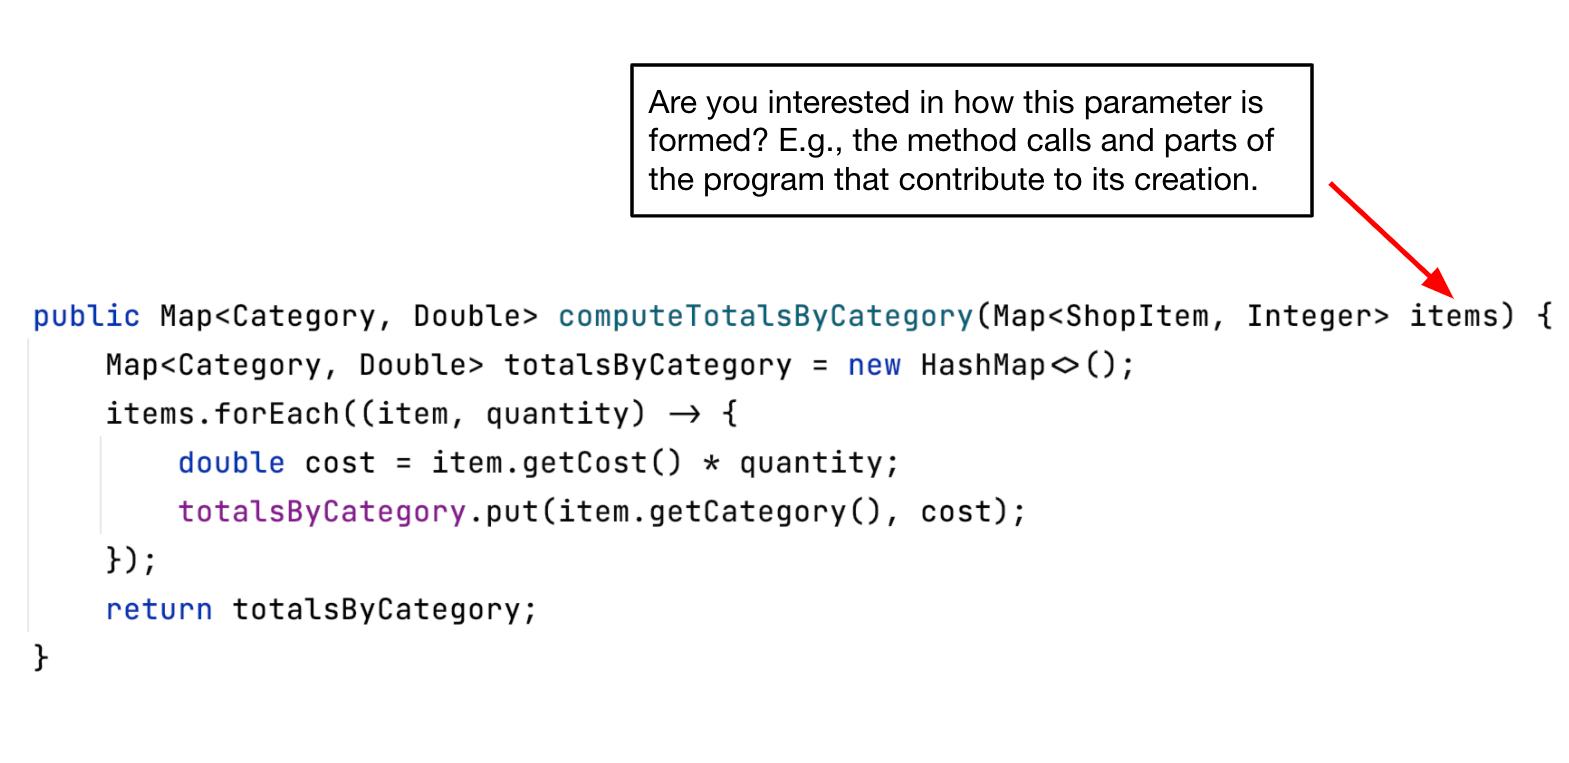
\includegraphics[width=\textwidth]{./figs/ds1.png}
\label{fig:DS1}
\end{figure}

\subsection{Development Scenario 2}

\begin{itemize}
  \item[] \textbf{Question text:} This figure (Figure \ref{fig:DS2}) represents 
          a scenario where a developer is rewriting a method. The code on the 
          left is the method before the developer made changes, while the one 
          on the right is an updated version.
  \item[] \textbf{Question presented to participant:}  \\
         ``Did I introduce any unwanted changes in the new version of this 
           code?"
\end{itemize}

\begin{figure}[ht]
\centering
\caption{Development Scenario 2}
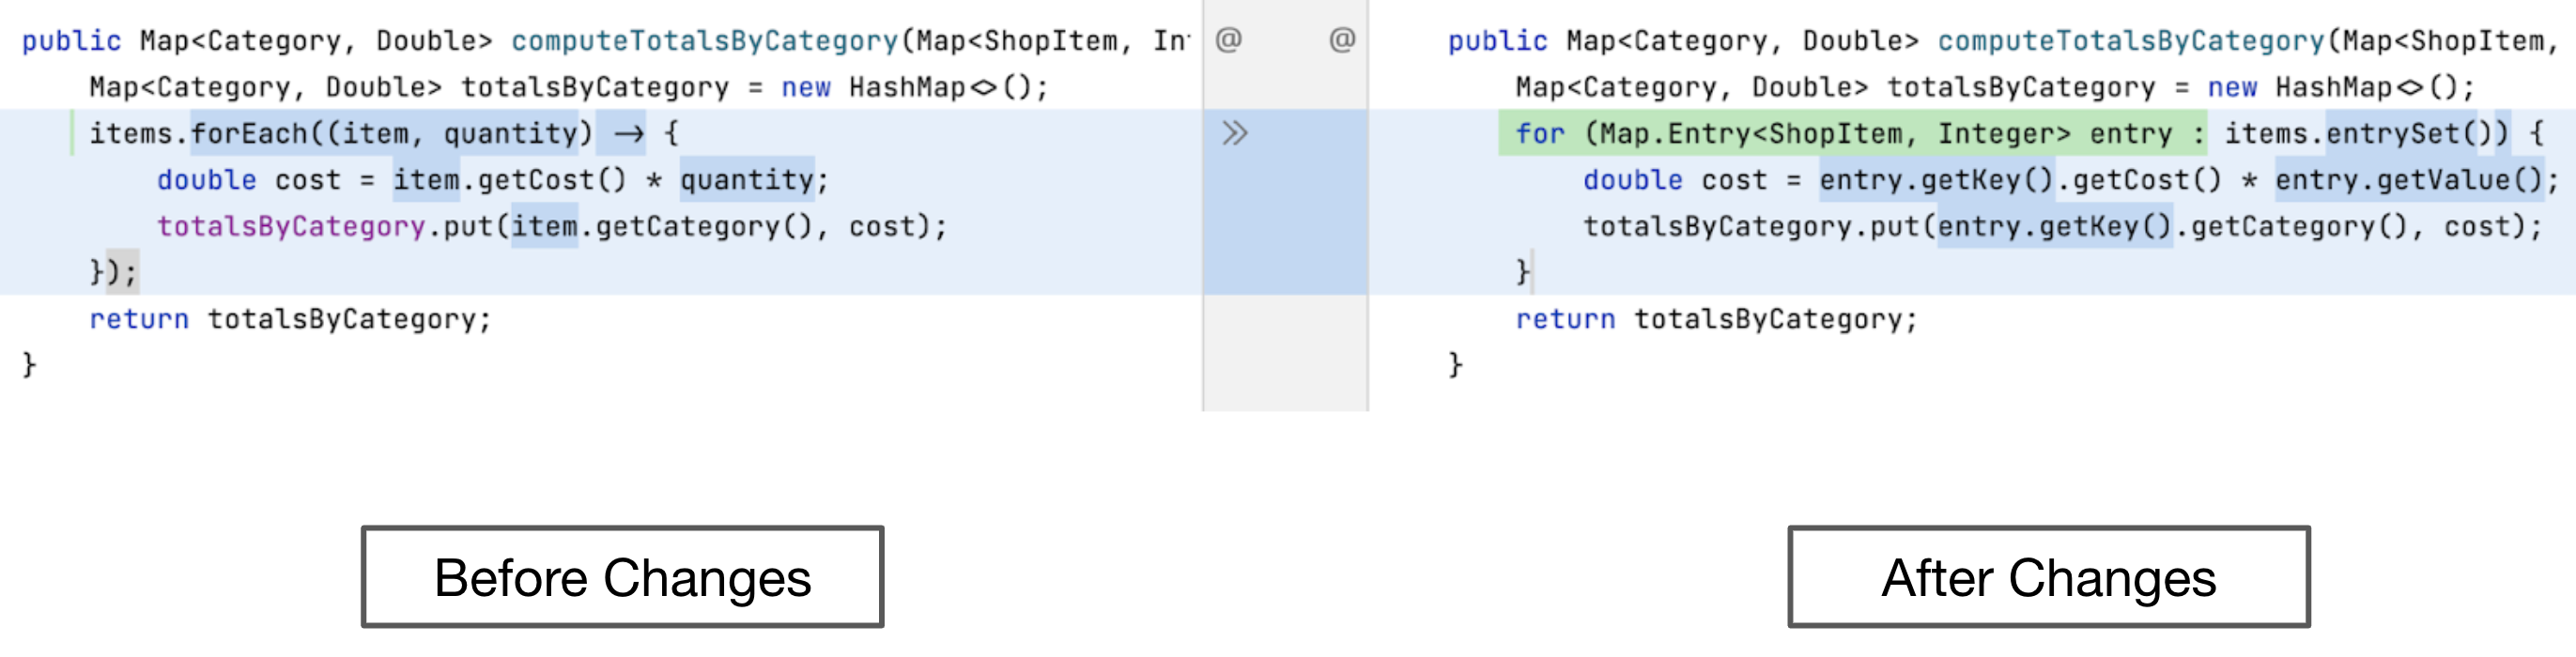
\includegraphics[width=\textwidth]{./figs/ds2.png}
\label{fig:DS2}
\end{figure}

\subsection{Development Scenario 3}

\begin{itemize}
  \item[] \textbf{Question text:} This figure (Figure \ref{fig:DS3}) represents 
          a scenario where an object is constructed within a method. The 
          implementation of the constructor and the various sources of data 
          used in creating the object, may not be immediately clear.
  \item[] \textbf{Question presented to participant:}  \\
          ``How is an instance of this class (in this case, 
           \texttt{ShoppingCart}) created/initialized?"
\end{itemize}

\begin{figure}[ht]
\centering
\caption{Development Scenario 3}
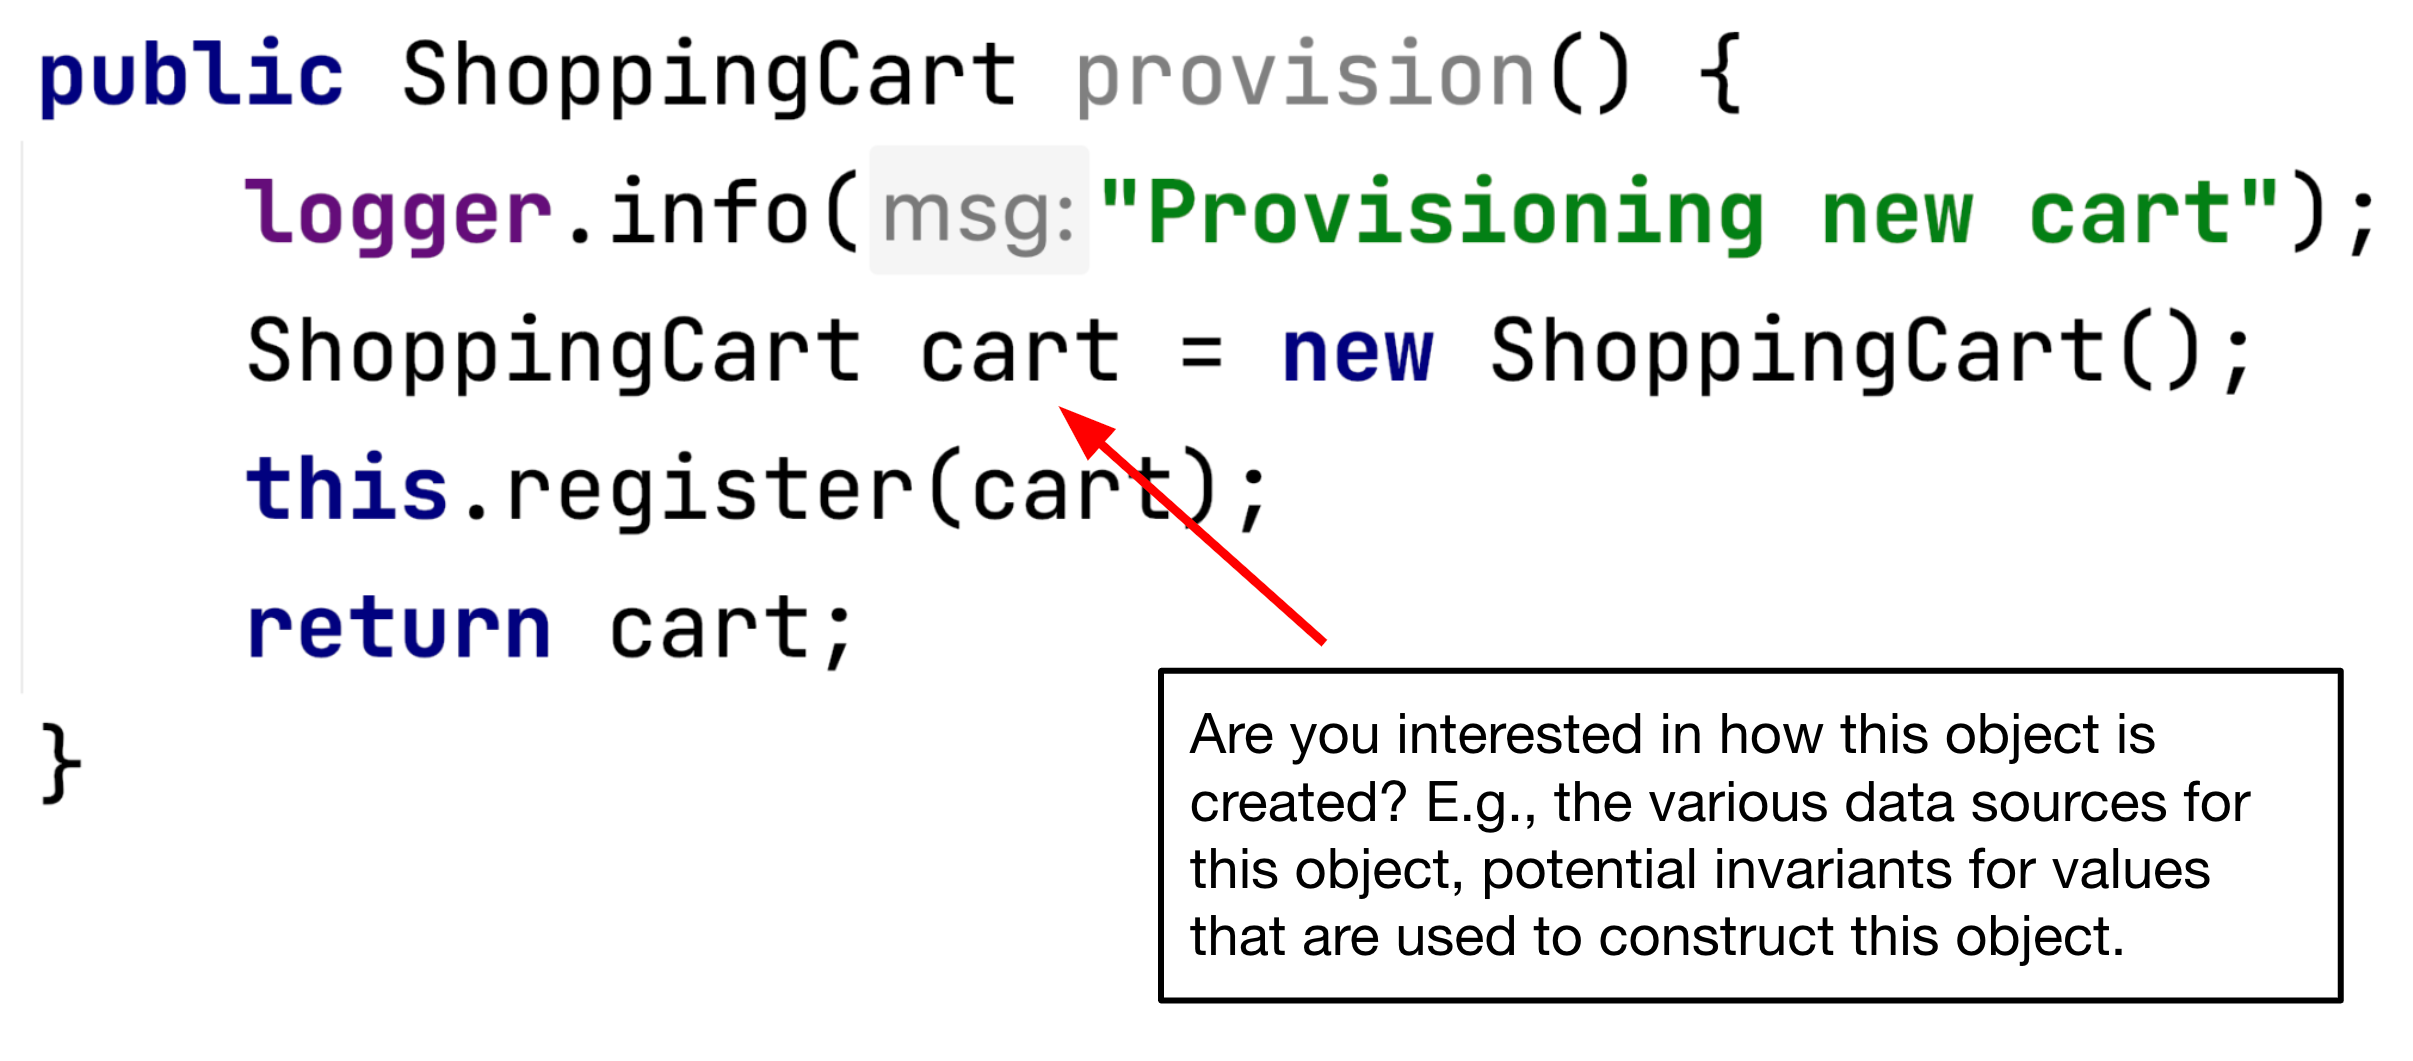
\includegraphics[width=\textwidth]{./figs/ds3.png}
\label{fig:DS3}
\end{figure}

\subsection{Development Scenario 4}

\begin{itemize}
  \item[] \textbf{Question text:} This figure (Figure \ref{fig:DS4}) represents 
          a scenario where some data is created (the \textbf{cart} object), and
          passed along as an argument to some methods. It may not be 
          immediately clear how this data is being \textbf{accessed} (\eg 
          which fields of the \textbf{cart} object are being used).
  \item[] \textbf{Question presented to participant:}  \\
          ``Given some data (in this case, \textbf{cart}), which parts of it
          are \textbf{accessed} downstream?"
\end{itemize}

\begin{figure}[ht]
\centering
\caption{Development Scenario 4}
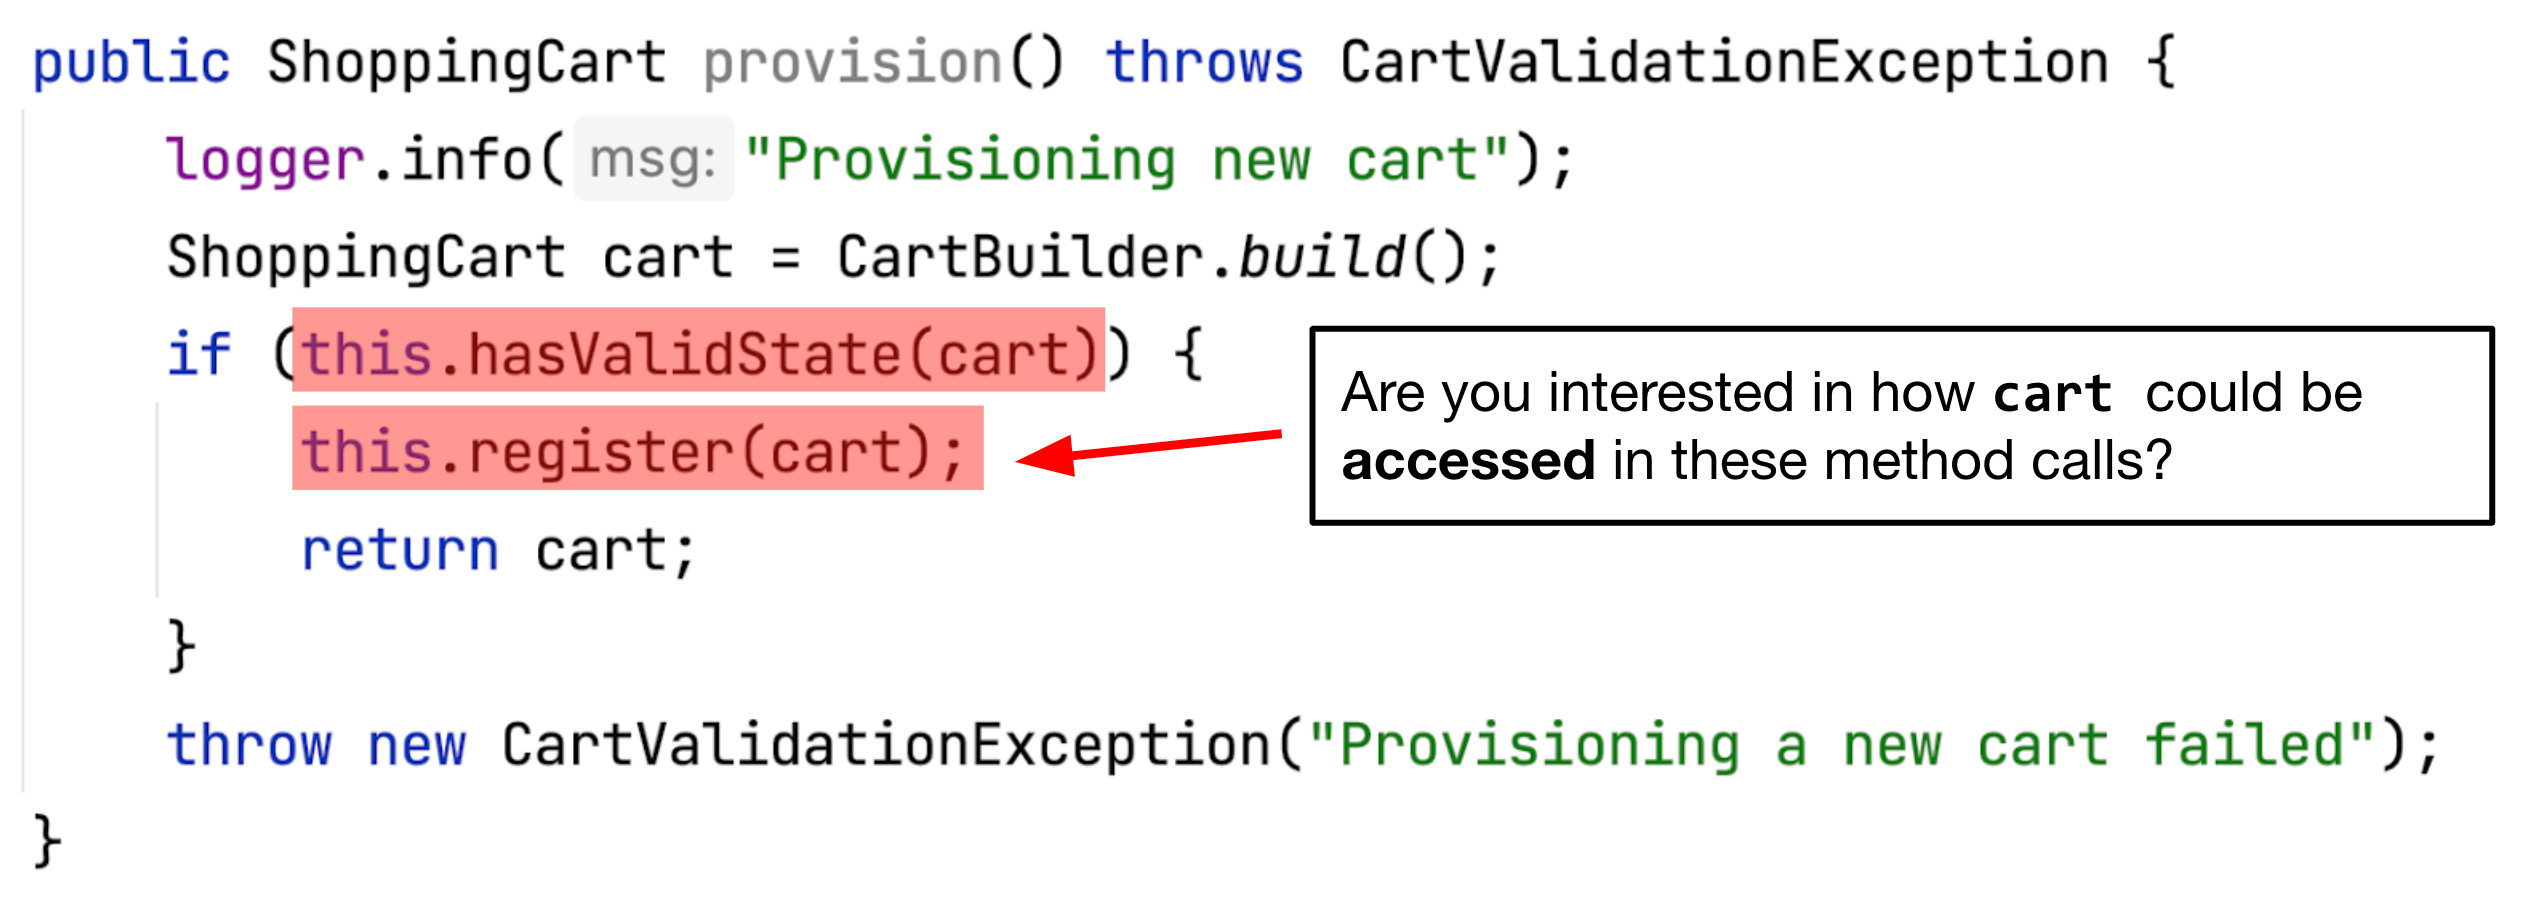
\includegraphics[width=\textwidth]{./figs/ds4.png}
\label{fig:DS4}
\end{figure}

\subsection{Development Scenario 5}

\begin{itemize}
  \item[] \textbf{Question text:} This figure (Figure \ref{fig:DS5}) represents 
          a scenario where some data is created (the \textbf{cart} object), and
          passed along as an argument to some methods. It may not be 
          immediately clear how this data is being \textbf{modified} (\eg 
          which fields of the \textbf{cart} object are being modified or changed).
  \item[] \textbf{Question presented to participant:}  \\
          ``Given some data (in this case, \textbf{cart}), which parts of it
          are \textbf{modified} downstream?"
\end{itemize}

\begin{figure}[ht]
\centering
\caption{Development Scenario 5}
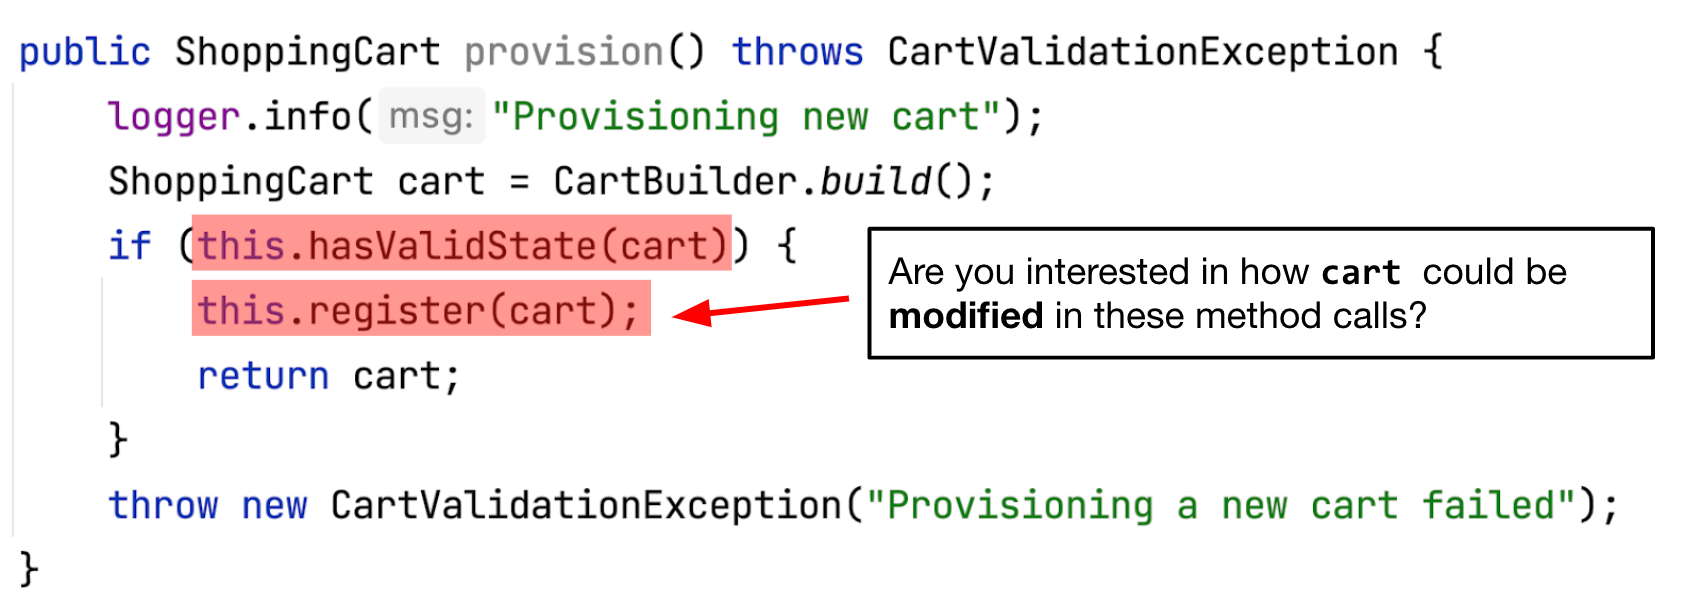
\includegraphics[width=\textwidth]{./figs/ds5.png}
\label{fig:DS5}
\end{figure}

\subsection{Development Scenario 6}

\begin{itemize}
  \item[] \textbf{Question text:} This figure (Figure \ref{fig:DS6}) represents 
          a scenario where a developer inspects a method. A popup appears that 
          notifies them that the method being inspected is not used anywhere in 
          the codebase.
  \item[] \textbf{Question presented to participant:}  \\
         ``Is deleting what appears to be unused code (in this case, 
         \textbf{transferItems}) going to break anything?"
\end{itemize}

\begin{figure}[ht]
\centering
\caption{Development Scenario 6}
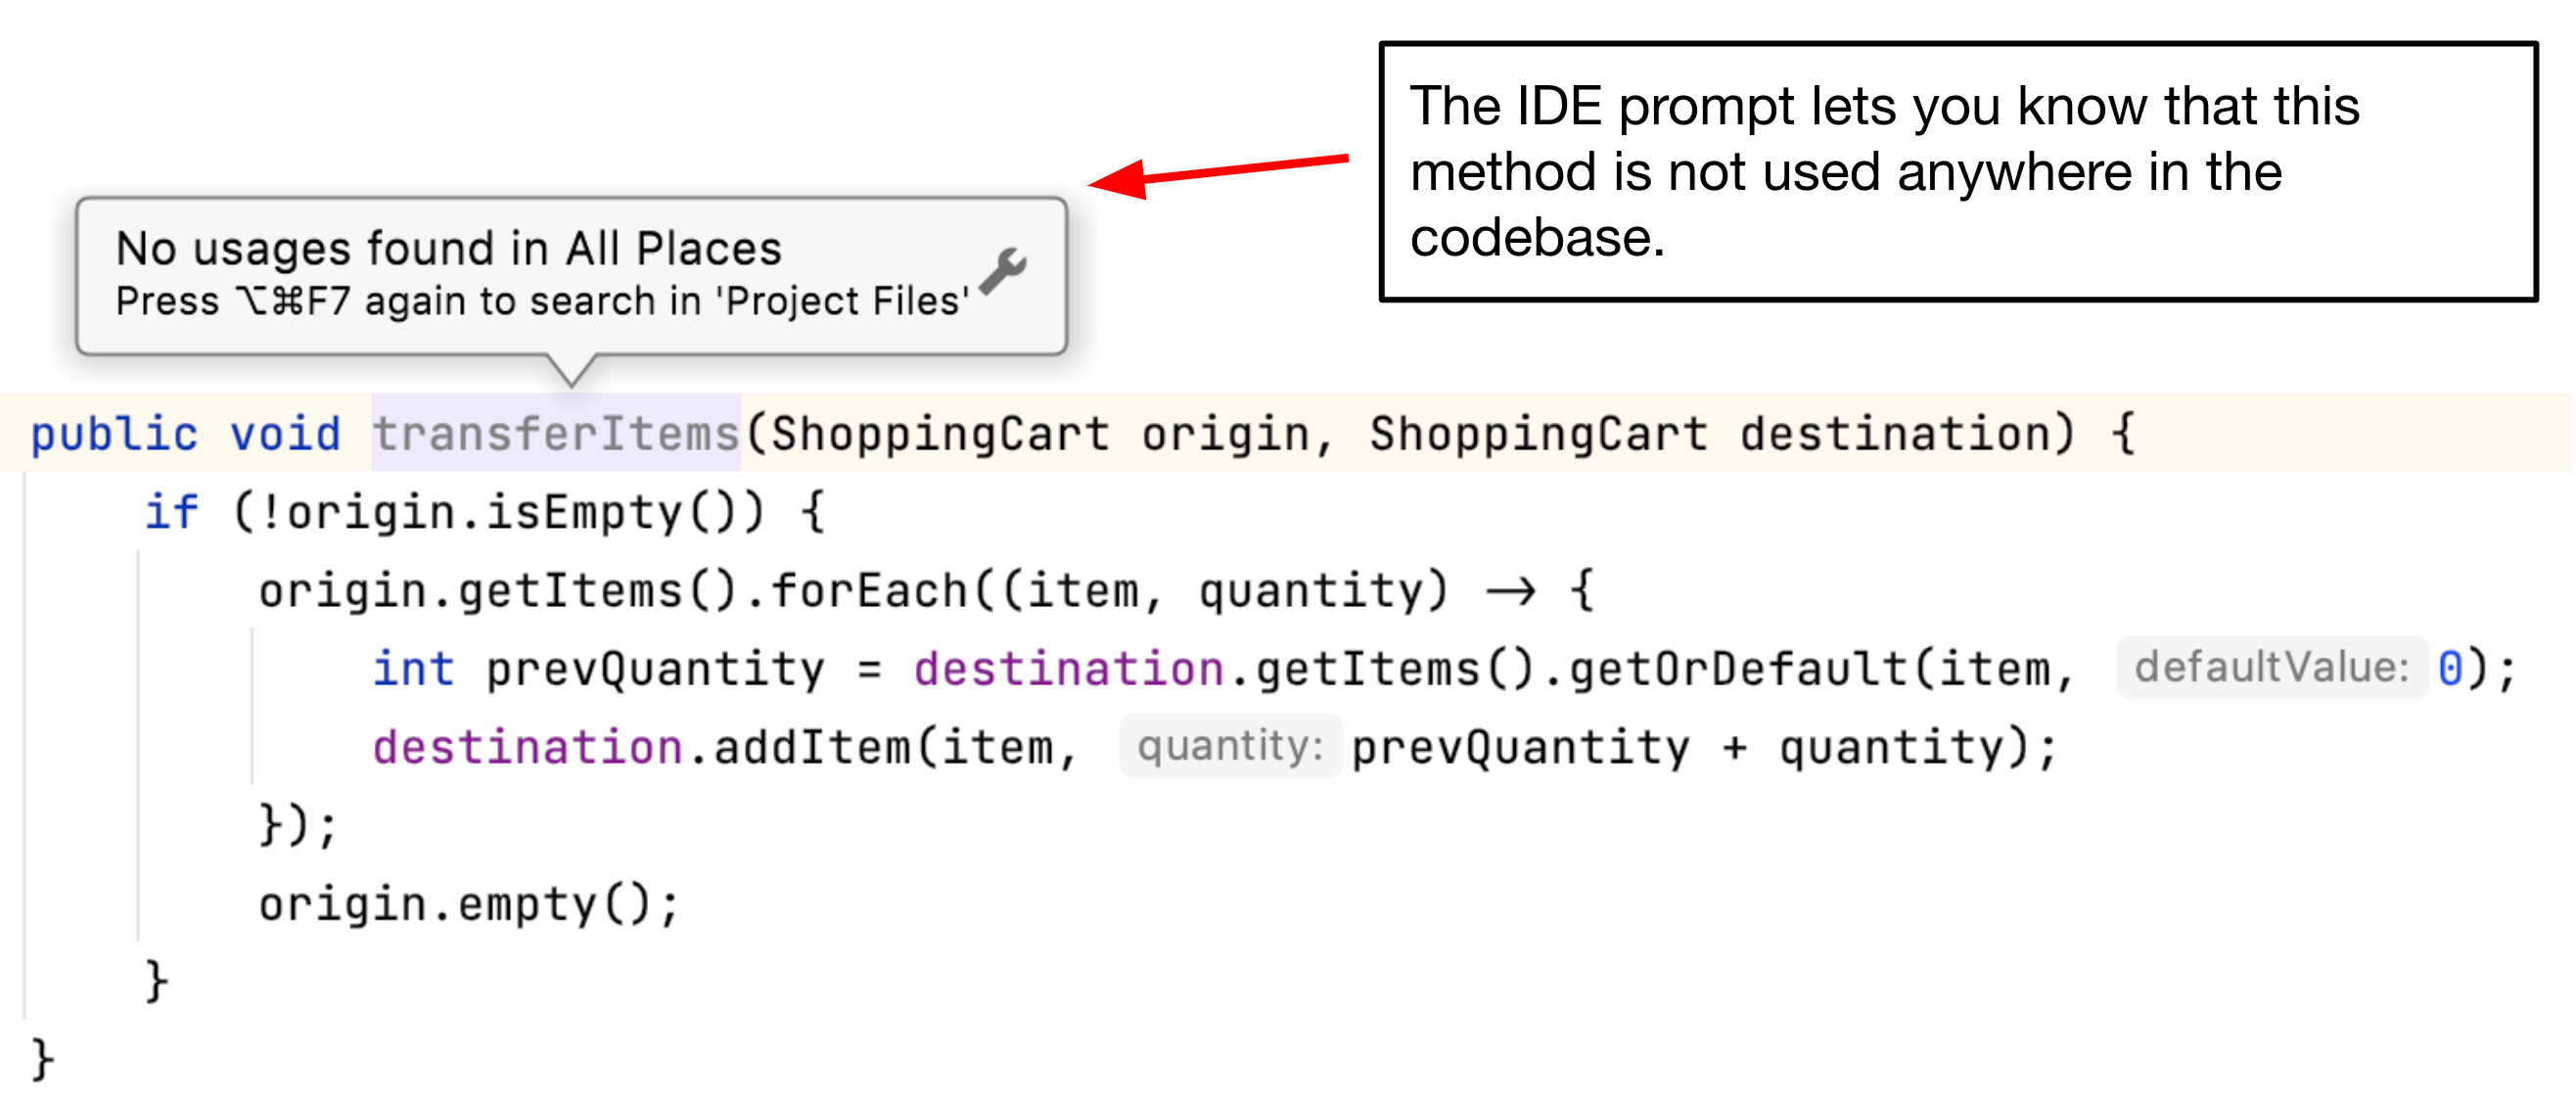
\includegraphics[width=\textwidth]{./figs/ds6.png}
\label{fig:DS6}
\end{figure}

\subsection{Development Scenario 7}

\begin{itemize}
  \item[] \textbf{Question text:} In this scenario, a developer may be 
          inspecting an interface. They are interested in how the method 
          \textbf{provision} may be implemented. A popup window shows that 
          there are two subtypes of the interface that implement 
          \textbf{provision}.
  \item[] \textbf{Question presented to participant:}  \\
          ``Given two subtypes and their implementations of a common method 
          (in this case, \textbf{provision}), how do they handle data 
          differently?"
\end{itemize}

\begin{figure}[ht]
\centering
\caption{Development Scenario 7}
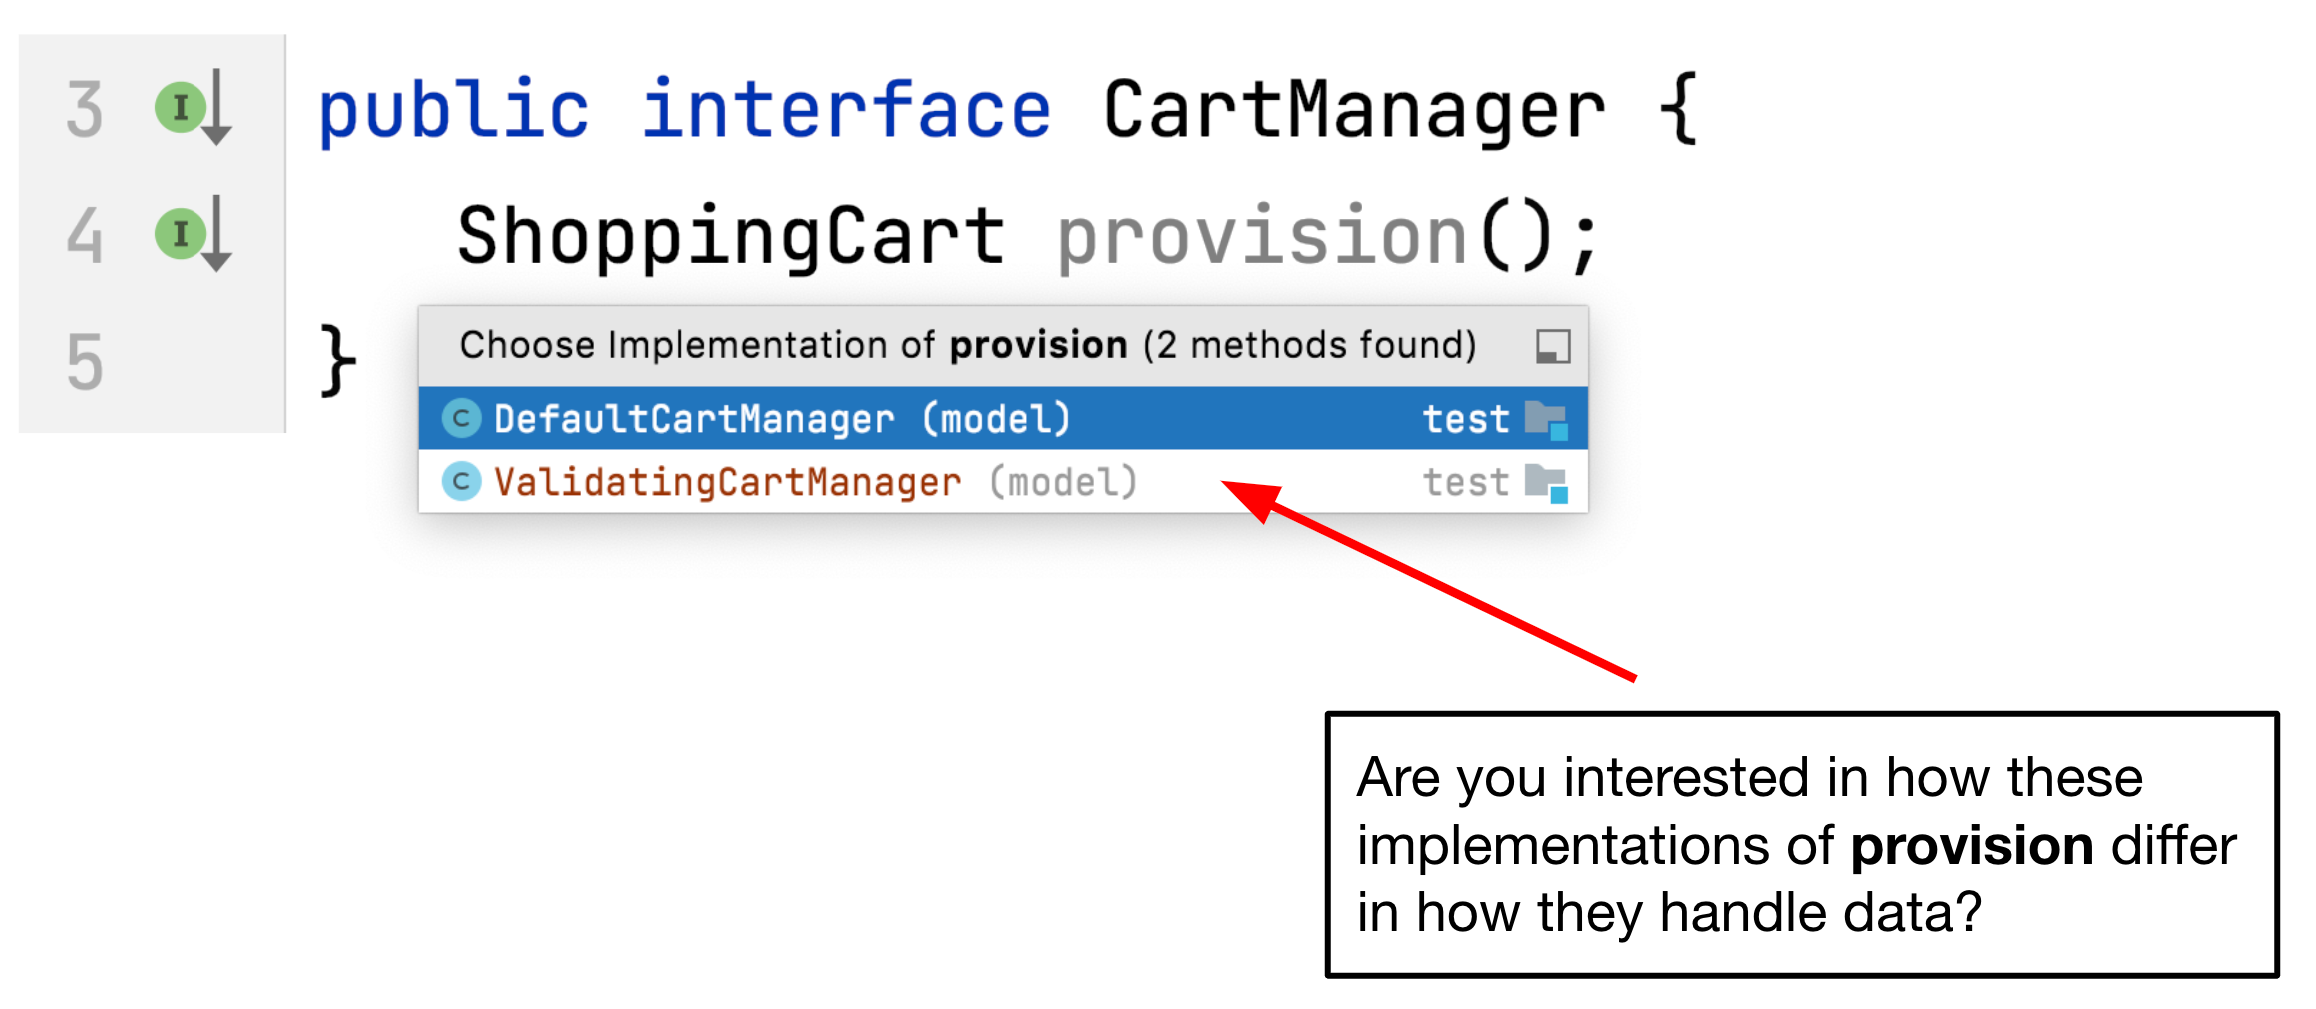
\includegraphics[width=\textwidth]{./figs/ds7.png}
\label{fig:DS7}
\end{figure}

\subsection{Development Scenario 8}

\begin{itemize}
  \item[] \textbf{Question text:} This figure (Figure \ref{fig:DS8}) shows a 
          method with a conditional statement (code within the branches are 
          omitted). This is a scenario where control-flow is \textbf{dependent} 
          on the value of data that a method is operating on. 
          A similar scenario might be a switch statement.
\item[] \textbf{Question presented to participant:}  \\
         ``Given some part of a program that depends on a value, which parts of 
         it are executed or reachable?"
\end{itemize}

\begin{figure}[ht!]
\centering
\caption{Development Scenario 8}
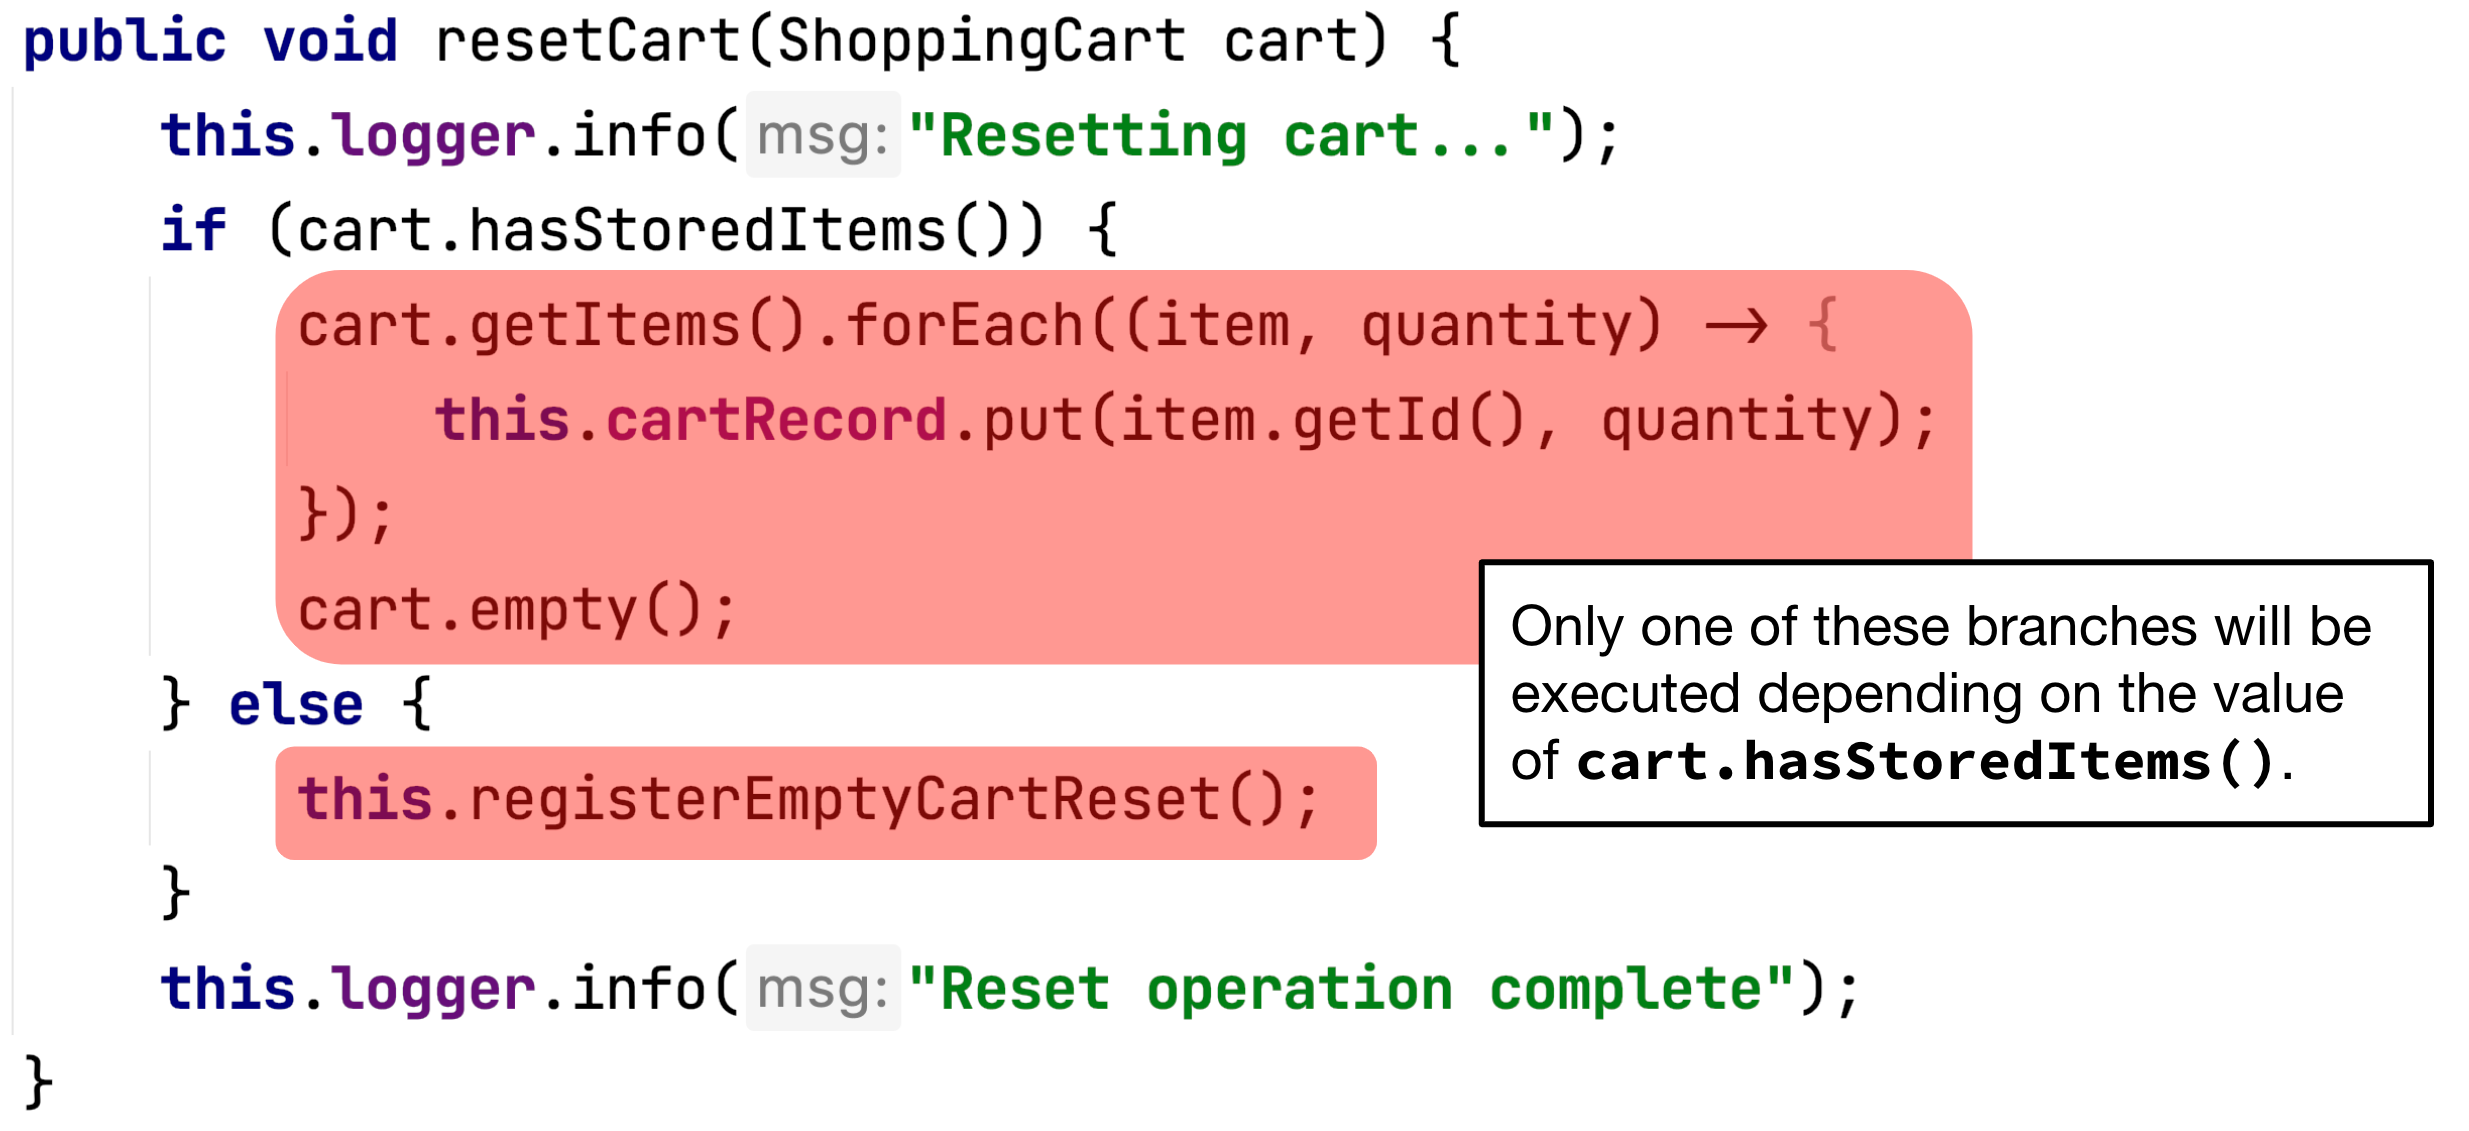
\includegraphics[width=\textwidth]{./figs/ds8.png}
\label{fig:DS8}
\end{figure}

\pagebreak

\subsection{Development Scenario 9}

\begin{itemize}
  \item[] \textbf{Question text:} A developer is inspecting a method and its 
          call hierarchy. She begins to read it line-by-line, and click through 
          other method calls that are within it (\eg jump to method 
          implementation). She continues this process until she eventually 
          arrives at a location where she wants to stop.

         \par Having navigated through a number of methods to arrive at this 
         location, she wants to trace back to where she started to synthesize a 
         high-level overview of the statements between the method where she 
         started, and the location in code where she ended.
  \item[] \textbf{Question presented to participant:}  \\
         ``What does the control-flow look like between two locations in code?"
\end{itemize}
